%%%%%%%%%%%%%%%%%%%%%%%%%%%%% Define Article %%%%%%%%%%%%%%%%%%%%%%%%%%%%%%%%%%
\documentclass[UTF8, 12pt]{ctexart}
%%%%%%%%%%%%%%%%%%%%%%%%%%%%%%%%%%%%%%%%%%%%%%%%%%%%%%%%%%%%%%%%%%%%%%%%%%%%%%%

%%%%%%%%%%%%%%%%%%%%%%%%%%%%% Using Packages %%%%%%%%%%%%%%%%%%%%%%%%%%%%%%%%%%
\usepackage{geometry}
\usepackage{graphicx}
\usepackage{mdframed}
\usepackage{booktabs}
\usepackage{color}
\usepackage{psfrag}
\usepackage{pdfpages}
\usepackage{float}
\usepackage{hyperref}
\usepackage{minted}
\usepackage{subfiles}
%%%%%%%%%%%%%%%%%%%%%%%%%%%%%%%%%%%%%%%%%%%%%%%%%%%%%%%%%%%%%%%%%%%%%%%%%%%%%%%

% Other Settings
\definecolor{shallowYellow}{RGB}{106,82,56}
\hypersetup{hypertex=true,
bookmarks=true,
bookmarksnumbered=true,
%hidelinks,
colorlinks=true,
linkcolor=shallowYellow,
anchorcolor=shallowYellow,
citecolor=shallowYellow,
urlcolor=shallowYellow,
pdftitle={Deauthentication Flood Attack},
pdfauthor={objout},
pdfsubject={Wireless Network Security},
pdfkeywords={WLAN Security,Deauth Flood Attack,Open Source},
pdfstartview=Fit,
pdfcreator={objout},
pdfproducer={objout}}

% 代码
%\usepackage{listings}
%\lstset{
%basicstyle=\ttfamily,
%keywordstyle=\bfseries,
%commentstyle=\rmfamily\itshape,
%stringstyle=\ttfamily,
%flexiblecolumns,
%numbers=left,
%showspaces=false,
%numberstyle=\zihao{-5}\ttfamily,
%showstringspaces=false,
%captionpos=t,
%frame=lrtb,
%}

%\PassOptionsToPackage{AutoFakeBold}{xeCJK}
%\PassOptionsToPackage{quiet}{fontspec}

\graphicspath{{figures/}}

\usepackage{indentfirst}
\setlength{\parindent}{2em}

%%%%%%%%%%%%%%%%%%%%%%%%%% Page Setting %%%%%%%%%%%%%%%%%%%%%%%%%%%%%%%%%%%%%%%
\setcounter{tocdepth}{4}
\setcounter{secnumdepth}{4}
% 设置四级目录与标题

%%%%%%%%%%%%%%%%%%%%%%%%%%%%%%% Title & Author %%%%%%%%%%%%%%%%%%%%%%%%%%%%%%%%
\title{Deauth Flood 攻防}
\author{胡嘉鑫 \and 张超祥 \and 许诚龙 \and 方赞}
\date{\today}
%%%%%%%%%%%%%%%%%%%%%%%%%%%%%%%%%%%%%%%%%%%%%%%%%%%%%%%%%%%%%%%%%%%%%%%%%%%%%%%

\begin{document}
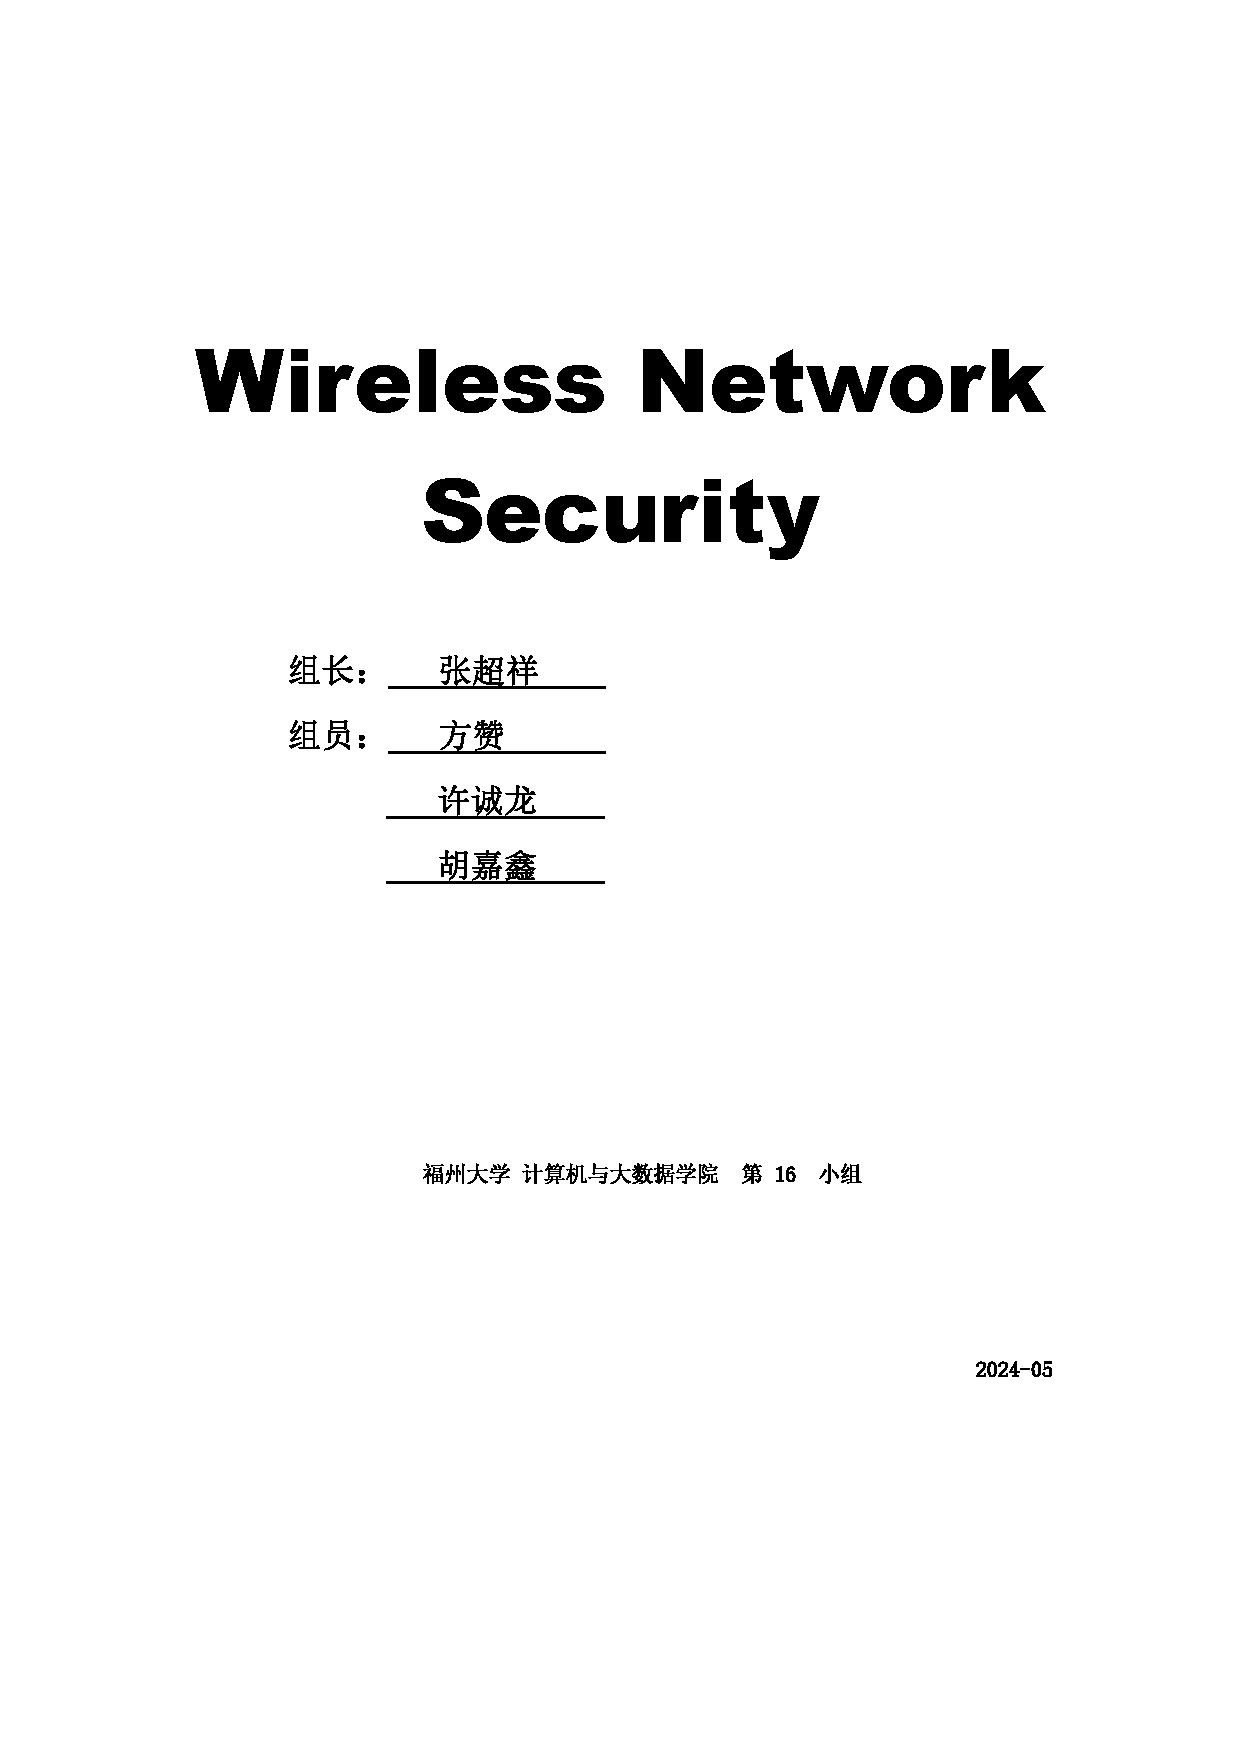
\includepdf[pages={1-1}]{./assets/cover.pdf}
\maketitle
\begin{abstract}
  本文涵盖了无线网络安全领域的工具和概念,重点介绍了 Deauthentication
  (Deauth)攻击及相关工具。esp8266\_deauther 是一个开源项目,
  允许用户在无线网络中对设备进行 Deauth 攻击。该项目提供用户友好的界面,
  除 Deauth攻击外,还可以监控无线网络流量等功能。
  此外,文中还介绍了 Arduino IDE,这是一个支持多个操作系统的开发工具,
  具有代码编辑、串口监控、库管理和编译等功能。
  还提及了安信可串口调试助手,用于调试串行通信过程。
  本文解释了无线网络通信原理,重点介绍了无线网络通信的
  组件和工作原理。详细阐述了Deauth Flood Attack,
  一种常见的无线网络攻击,会中断设备与访问点的连接,
  可能导致服务中断或不稳定。文中还提到了防御 Deauth 攻击的步骤,
  如使用加密协议、监视网络流量和限制无线网络访问。

  实验中介绍了硬件和软件的准备工作,包括PC、ESP8266 Wi-Fi模块、
  Arduino IDE、安信可串口调试助手、Flash Download Tool、esp8266\_deauther等工具。
  提供了编译和生成 ESP8266 上执行固件的步骤,包括运行 Arduino CLI 编译脚本以生成bin文件,
  并使用Flash Download Tool上传到 ESP8266 的过程。随后详细说明了在 ESP8266
  设备上执行 Deauth 攻击的步骤,包括确认客户端(受害者)连接到访问点(AP)、
  使用安信可串口调试助手扫描附近通信、攻击者选择受害者客户端并发动攻击,
  使受害者下线。最后,给出了防范措施。
\end{abstract}

\textbf{关键词}: WLAN Security、Deauth Flood Attack、Cyberspace Security.

\newpage
\tableofcontents
\newpage
\subfile{./sections/1_实验背景.tex}
\subfile{./sections/2_实验目的.tex}
\subfile{./sections/3_实验环境.tex}
\subfile{./sections/4_实验工具.tex}
\subfile{./sections/5_实验原理.tex}
\subfile{./sections/6_实验步骤.tex}
\subfile{./sections/7_防范措施.tex}
\subfile{./sections/8_实验总结.tex}
\subfile{./sections/9_免责声明.tex}
\end{document}
